\documentclass[11pt,a4paper]{article}
\usepackage[T1]{fontenc}
\usepackage[margin=2.3cm]{geometry}
\usepackage{amsmath,amssymb}
\usepackage{graphicx}
\usepackage[dvipsnames]{xcolor}
\usepackage{enumitem}
\usepackage[colorlinks=true,linkcolor=blue,urlcolor=blue]{hyperref}
\setlength{\parskip}{0.6em}
\setlength{\parindent}{0pt}
\begin{document}

\begin{center}{\LARGE\bfseries openphtitration}\\[0.4em]{\large Find an unknown acid concentration from a titration curve, in three sessions.}\\[0.2em]\small PAN IIT OSS explainer \textbullet{} secondary school to diploma / undergraduate (levels 3-5)\end{center}

\section*{Why this exists}
A titration finds an unknown concentration by adding a known solution until the two exactly cancel. The pH of the flask changes slowly and then suddenly, and that sudden change tells you how much was needed. This explainer shows the mathematics behind it with logarithms, a mole balance and a numerical root finder.

\section*{The end goal}
Find an unknown acid concentration from a titration curve. The end goal is finding an unknown acid concentration from a titration curve: computing the curve for strong and weak acids, checking it against simple formulas, and locating the equivalence point in noisy data. The same methods are used in water testing, food analysis and pharmaceutical quality control. This is a simulation for education; real acids and bases need supervision.

\section*{How the three sessions build up}
\begin{enumerate}[nosep]
\item \textbf{Session 1: Acids, bases and the shape of a titration curve} (Level 1, conceptual interactive model, 60 min).
\item \textbf{Session 2: pH, pOH and the mathematics of the strong acid - strong base curve} (Level 2, mathematical engineering model, 75 min).
\item \textbf{Session 3: Weak acids: buffers, the numerical curve and the noisy endpoint} (Level 3, simulation and validation, 90 min).
\end{enumerate}

\section{Session 1: Acids, bases and the shape of a titration curve}

\subsection*{A. Real-world problem}
A lab has a bottle of acid and needs to know how strong it is. They cannot taste it and the label is gone. So they add a base of known strength from a glass tube (a burette), a little at a time, and watch the liquid in the flask. At first almost nothing seems to happen; then, with one more drop, everything changes. How does that sudden change reveal the strength of the acid? This is general education about a simulation: real acids and bases must only be handled with a teacher, goggles and the right equipment.

\subsection*{B. Concept and theory}
Water always contains a few hydrogen ions (H+). An acid adds more of them, a base removes them. The pH is the number that measures this: pH = -log10[H+], where [H+] is the concentration of hydrogen ions in mol/L. Because of the logarithm, a drop of 1 in pH means ten times more H+. A solution with pH below 7 is acidic, 7 is neutral (pure water at 25 C) and above 7 is basic. A strong acid such as hydrochloric acid (HCl) splits completely, so 0.1 mol/L HCl has [H+] = 0.1 and pH 1. In a titration we add base of known concentration Cb from a burette to Va mL of acid of concentration Ca. Acid and base cancel mole for mole. While acid is left over, the pH is low. Exactly when the moles of base added equal the moles of acid, we are at the equivalence point; just past it, base is left over and the pH is high. The leftover is divided by the total volume, so the pH changes slowly while there is plenty of acid and very fast when the leftover is tiny.

\begin{itemize}[nosep]
\item pH: measure of acidity, -log10[H+] (no unit)
\item [H+]: concentration of hydrogen ions (mol/L)
\item Ca, Va: concentration and volume of the acid in the flask (mol/L, mL)
\item Cb, Vb: concentration and volume of the base added (mol/L, mL)
\item Ve: equivalence volume: base needed to cancel all the acid (mL)
\end{itemize}

\begin{equation*}
\mathrm{pH}=-\log_{10}[\mathrm{H}^+]
\end{equation*}

\begin{equation*}
x=\frac{C_aV_a-C_bV_b}{V_a+V_b}\quad(\text{leftover acid if }x>0,\ \text{leftover base if }x<0)
\end{equation*}

\begin{equation*}
C_aV_a=C_bV_e\quad\Rightarrow\quad V_e=\frac{C_aV_a}{C_b}
\end{equation*}

\begin{center}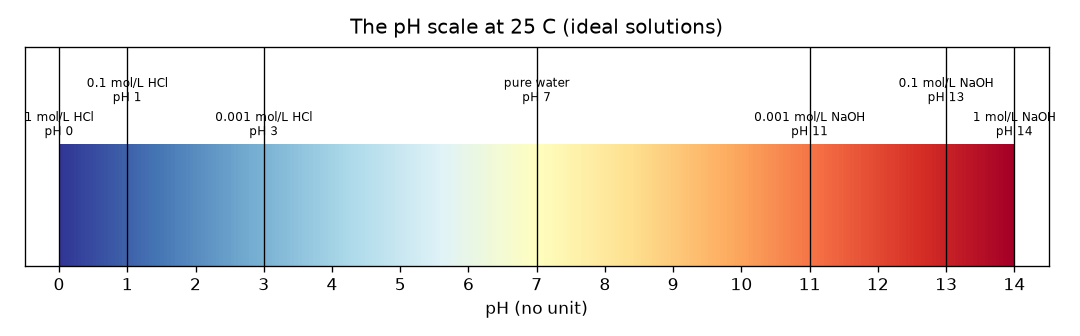
\includegraphics[width=0.85\linewidth]{figures/s01_ph_scale.png}\\\small The pH scale from 0 to 14 with strong acid and base solutions placed on it.\end{center}

\subsection*{E. Worked example}
25 mL of 0.1 mol/L HCl is titrated with 0.1 mol/L NaOH. Find the pH after 10 mL of base, and the equivalence volume.
\begin{enumerate}[nosep]
\item Moles of acid at the start: 0.1 mol/L x 25 mL = 2.5 mmol.
\item Moles of base added: 0.1 mol/L x 10 mL = 1.0 mmol. They cancel one for one, so 2.5 - 1.0 = 1.5 mmol of acid is left.
\item Total volume = 25 + 10 = 35 mL, so [H+] = 1.5 / 35 = 0.04286 mol/L.
\item pH = -log10(0.04286) = 1.368.
\item Equivalence: Ca Va = Cb Ve gives Ve = 0.1 x 25 / 0.1 = 25 mL, where only water and salt are left and pH = 7.
\end{enumerate}
\textbf{Answer.} After 10 mL the pH is 1.368; the equivalence volume is 25 mL (pH 7).

\subsection*{F. Questions}
\begin{enumerate}[nosep]
\item \textbf{Conceptual.} Why does the pH hardly change for the first 20 mL of base and then jump within a fraction of a millilitre near 25 mL?
\item \textbf{Numerical.} What is the pH after 20 mL of 0.1 mol/L NaOH has been added to 25 mL of 0.1 mol/L HCl? Show the units and check that the answer is sensible.
\item \textbf{Graph and simulation interpretation.} On the titration curve, how much does the pH change between 24.9 mL and 25.1 mL, and what does that tell you about reading the burette near the end?
\item \textbf{Design and optimisation challenge.} Design: you have 25 mL of 0.1 mol/L acid and a choice of 0.1 mol/L or 0.2 mol/L base. Which do you choose and why? State the equivalence volume for each and the trade-off.
\end{enumerate}

\section{Session 2: pH, pOH and the mathematics of the strong acid - strong base curve}

\subsection*{A. Real-world problem}
A water-treatment student must find the strength of an acid sample and has two dyes: methyl orange and phenolphthalein. A wrong dye changes colour too early or too late and the answer is off. How do we compute the whole curve, turn the burette reading into a concentration, and pick a dye that is right for the job? As before, real chemicals need supervision: this is a simulation and general education.

\subsection*{B. Concept and theory}
Water always keeps [H+][OH-] = Kw = 1e-14 (mol/L)\textasciicircum{}2 at 25 C. Taking -log10 of both sides gives pH + pOH = 14. During a titration, the net leftover x = (Ca Va - Cb Vb)/(Va + Vb) is positive (acid left), zero (equivalence) or negative (base left). Including water, x = [H+] - Kw/[H+], so [H+] = (x + sqrt(x\textasciicircum{}2 + 4 Kw))/2. This one formula gives pH 1 at the start of 0.1 mol/L HCl, exactly 7 at equivalence (x = 0) and a high pH after it. At equivalence the moles balance, Ca Va = Cb Ve, so one burette reading gives the concentration: Ca = Cb Ve / Va. An indicator is a dye that changes colour over a short pH range. The colour changes at the volume where the flask pH is in that range, so we ask how far that volume is from Ve. Methyl orange changes at about pH 3.1 to 4.4 and phenolphthalein at about 8.2 to 10 (approximate, well-known ranges). Finally, diluting does not change the moles of dissolved acid: C1 V1 = C2 V2.

\begin{itemize}[nosep]
\item pH, pOH: -log10[H+], -log10[OH-] (no unit)
\item Kw: ion product of water, 1e-14 at 25 C ((mol/L)\textasciicircum{}2)
\item x: net leftover acid (+) or base (-) (mol/L)
\item Ca, Va: acid concentration and volume (mol/L, mL)
\item Cb, Vb, Ve: base concentration, volume added, equivalence volume (mol/L, mL, mL)
\item C1, V1, C2, V2: concentration and volume before and after dilution (mol/L, mL)
\end{itemize}

\begin{equation*}
\mathrm{pH}+\mathrm{pOH}=14\qquad([\mathrm{H}^+][\mathrm{OH}^-]=K_w=10^{-14})
\end{equation*}

\begin{equation*}
[\mathrm{H}^+]=\frac{x+\sqrt{x^2+4K_w}}{2},\qquad x=\frac{C_aV_a-C_bV_b}{V_a+V_b}
\end{equation*}

\begin{equation*}
C_aV_a=C_bV_e\quad\Rightarrow\quad C_a=\frac{C_bV_e}{V_a}
\end{equation*}

\begin{equation*}
V_b=\frac{C_aV_a-xV_a}{C_b+x}\quad(\text{volume at which the flask has a given pH, with }x=[\mathrm{H}^+]-K_w/[\mathrm{H}^+])
\end{equation*}

\begin{equation*}
C_1V_1=C_2V_2
\end{equation*}

\begin{center}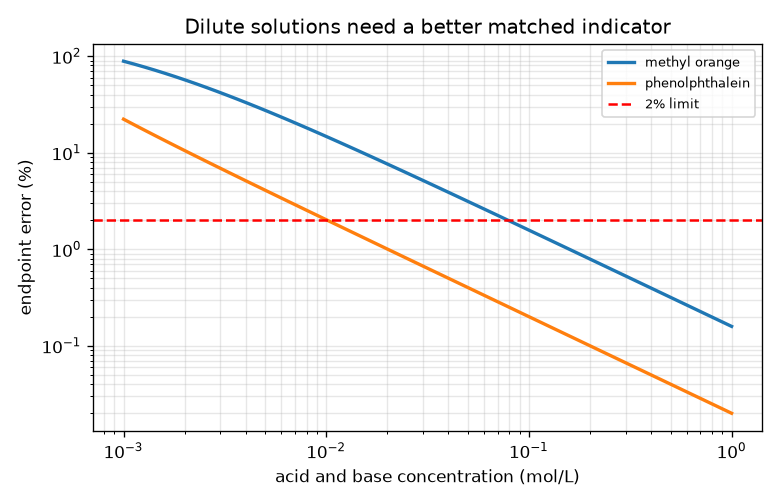
\includegraphics[width=0.85\linewidth]{figures/s02_indicator_error.png}\\\small Endpoint error against concentration for the two dyes; the red line is the 2 percent limit.\end{center}

\subsection*{E. Worked example}
A 25.00 mL sample of unknown HCl needs 20.00 mL of 0.1000 mol/L NaOH to reach the equivalence point. Find the concentration and the starting pH. Then find the pH 0.1 mL before and after equivalence for the 0.1 mol/L case.
\begin{enumerate}[nosep]
\item At equivalence, moles of acid = moles of base: Ca x 25.00 = 0.1000 x 20.00 = 2.000 mmol.
\item Ca = 2.000 / 25.00 = 0.0800 mol/L.
\item Starting pH = -log10(0.0800) = 1.097.
\item For 25 mL of 0.1 mol/L acid and 24.9 mL of base: x = 0.01 mmol / 49.9 mL = 2.004e-4 mol/L, so pH = 3.698.
\item For 25.1 mL: x = -0.01 / 50.1 = -1.996e-4 mol/L of OH-, so pOH = 3.700 and pH = 14 - 3.700 = 10.300.
\end{enumerate}
\textbf{Answer.} Ca = 0.0800 mol/L with a starting pH of 1.097; the pH is 3.698 at 24.9 mL and 10.300 at 25.1 mL.

\subsection*{F. Questions}
\begin{enumerate}[nosep]
\item \textbf{Conceptual.} Why does pH + pOH = 14 hold for every aqueous solution at 25 C, even for a solution of a base?
\item \textbf{Numerical.} A 25.00 mL sample of acid needs 18.60 mL of 0.1000 mol/L NaOH. What is the acid concentration? What volume of water must be added to 10.00 mL of that acid to dilute it to a quarter of its concentration?
\item \textbf{Graph and simulation interpretation.} In the plot of three curves, what do the three curves have in common and how do they differ? What does that mean for finding the equivalence point of a very dilute acid?
\item \textbf{Design and optimisation challenge.} Design: which indicator (methyl orange or phenolphthalein) is suitable for a titration of 0.05 mol/L HCl with 0.05 mol/L NaOH, with an endpoint error of 2 percent allowed? For phenolphthalein, below roughly what concentration does it stop being suitable?
\end{enumerate}

\section{Session 3: Weak acids: buffers, the numerical curve and the noisy endpoint}

\subsection*{A. Real-world problem}
Vinegar is acetic acid, a weak acid. Its titration curve differs from the strong-acid curve: it starts at a higher pH, has a long flat stretch (a buffer), and its equivalence point is above pH 7, so the indicator choice changes. Real burette readings are also noisy. How do we compute the whole curve numerically, test it against simple formulas, find the equivalence point from messy data and turn it into the strength of the vinegar? Simulation only: real vinegar titrations should still be done with a teacher.

\subsection*{B. Concept and theory}
A weak acid HA only partly splits: HA \textless{}-\textgreater{} H+ + A-, with Ka = [H+][A-]/[HA]. For acetic acid Ka is about 1.8e-5 (pKa = -log10 Ka = 4.74). If Ct is the total acid concentration and Na the sodium (from the base), charge neutrality says Na + [H+] = [OH-] + [A-], with [OH-] = Kw/[H+] and [A-] = Ct Ka/(Ka + [H+]). This is one equation in the unknown [H+]; its left side minus its right side rises steadily with pH, so it has exactly one root, which we find by bisection on the pH. Between the start and equivalence the flask holds both HA and A-, and the charge balance reduces to the Henderson-Hasselbalch relation pH = pKa + log10([A-]/[HA]); using moles, [A-]/[HA] = Cb Vb/(Ca Va - Cb Vb). At half-equivalence the two are equal and pH = pKa. At equivalence only A- is left and it makes the solution basic: [OH-] = sqrt(Kb C), Kb = Kw/Ka. The buffer capacity beta = dNa/dpH measures how much base the flask absorbs per pH unit; it is largest at pH = pKa. In a real run the volume reading and the pH reading are both noisy; the equivalence point is where dpH/dV is largest. Very dilute acids are a failure case: below about 1e-6 mol/L the water itself supplies H+ and the simple formula pH = -log10 C gives nonsense.

\begin{itemize}[nosep]
\item Ka, pKa: acid dissociation constant and its -log10 (mol/L, no unit)
\item Ct: total acid concentration in the flask, [HA] + [A-] (mol/L)
\item Na: sodium concentration from the base (mol/L)
\item h: hydrogen-ion concentration [H+] (mol/L)
\item beta: buffer capacity, dNa/dpH (mol/L per pH unit)
\item sigma\_V, sigma\_pH: standard deviations of volume and pH reading noise (mL, no unit)
\end{itemize}

\begin{equation*}
K_a=\frac{[\mathrm{H}^+][\mathrm{A}^-]}{[\mathrm{HA}]},\qquad \mathrm{p}K_a=-\log_{10}K_a
\end{equation*}

\begin{equation*}
N_a+h-\frac{K_w}{h}-\frac{C_tK_a}{K_a+h}=0\qquad(h=[\mathrm{H}^+],\ \text{solve for }h)
\end{equation*}

\begin{equation*}
\mathrm{pH}=\mathrm{p}K_a+\log_{10}\frac{C_bV_b}{C_aV_a-C_bV_b}
\end{equation*}

\begin{equation*}
\beta=\ln 10\left(h+\frac{K_w}{h}+\frac{C_tK_ah}{(K_a+h)^2}\right),\qquad \beta_{\max}=\frac{\ln 10}{4}C_t\ \text{at pH}=\mathrm{p}K_a
\end{equation*}

\begin{equation*}
V_e=\arg\max_V\frac{d\,\mathrm{pH}}{dV},\qquad C_{\mathrm{vinegar}}=\frac{C_bV_e}{V_a}\times\text{dilution factor}
\end{equation*}

\begin{center}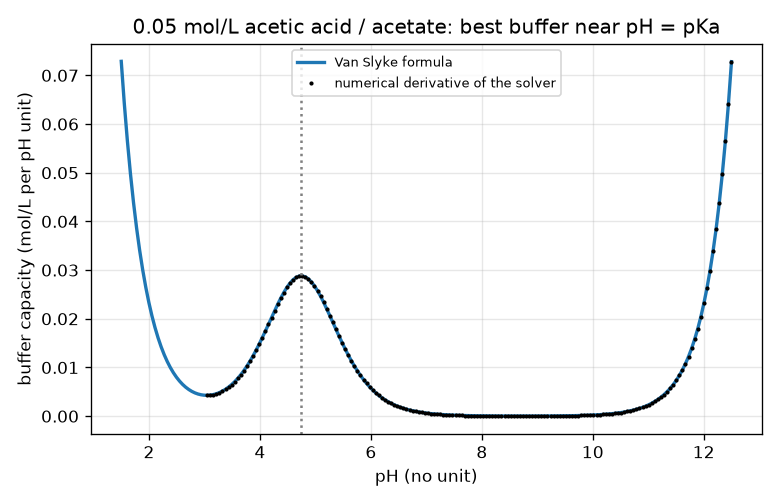
\includegraphics[width=0.85\linewidth]{figures/s03_buffer_capacity.png}\\\small Buffer capacity: the analytic formula and the numerical derivative of the solver agree, with a maximum at pH = pKa.\end{center}

\subsection*{E. Worked example}
25 mL of 0.1 mol/L acetic acid (Ka = 1.8e-5) is titrated with 0.1 mol/L NaOH. Find the pH after 10 mL by Henderson-Hasselbalch, compare with the exact numerical value, and find the equivalence pH.
\begin{enumerate}[nosep]
\item pKa = -log10(1.8e-5) = 4.745.
\item Moles: acid 0.1 x 25 = 2.5 mmol; base 0.1 x 10 = 1.0 mmol. After reaction n(A-) = 1.0 mmol and n(HA) = 2.5 - 1.0 = 1.5 mmol.
\item Henderson-Hasselbalch: pH = 4.745 + log10(1.0/1.5) = 4.745 - 0.176 = 4.569.
\item The bisection solver of the charge balance gives 4.569 as well (difference below 0.001).
\item Equivalence is at 25 mL: Ct = 2.5/50 = 0.05 mol/L of A-, Kb = 1e-14/1.8e-5 = 5.56e-10, [OH-] = sqrt(5.56e-10 x 0.05) = 5.27e-6 mol/L, pOH = 5.28, pH = 8.72. The solver gives 8.722.
\end{enumerate}
\textbf{Answer.} After 10 mL the pH is 4.569 (formula and solver agree); the equivalence point is at 25 mL with pH 8.72, above 7.

\subsection*{F. Questions}
\begin{enumerate}[nosep]
\item \textbf{Conceptual.} Why does a weak acid titration have a flat region around pH = pKa, and why is the equivalence point above 7 although acid and base have cancelled exactly?
\item \textbf{Numerical.} For the 0.1 mol/L acetic acid titration above, find the pH after 20 mL of base with Henderson-Hasselbalch. Then state the pH at 12.5 mL without calculating.
\item \textbf{Graph and simulation interpretation.} In the Henderson-Hasselbalch comparison table, where does the formula fail and why? Which direction does it err?
\item \textbf{Design and optimisation challenge.} Design: a student must locate the equivalence point of a vinegar titration with a volume reading noise of 0.03 mL and pH noise of 0.02. Compare a 1.0 mL step with a 0.2 mL step and recommend a plan. What does a 0.5 percent target on the concentration require?
\end{enumerate}

\section{Real-world mini-project}
\textbf{Find the acid in a bottle of vinegar.} Vinegar is about 5 g of acetic acid per 100 mL, which is 0.833 mol/L (molar mass 60.05 g/mol). A student dilutes 10.00 mL of vinegar to 100.00 mL, puts 25.00 mL of the dilution in a flask and titrates with 0.1000 mol/L NaOH, reading the burette every 0.2 mL. The readings have a volume noise of 0.03 mL and a pH noise of 0.02. Use \texttt{make\_data} from Session 3 to generate the synthetic run (diluted concentration 0.0833 mol/L, pKa from \texttt{PKA\_ACETIC}, volumes 0 to 35 mL), find the equivalence volume with \texttt{find\_equivalence}, then use \texttt{vinegar\_concentration} and \texttt{vinegar\_percent} to report the vinegar strength.

\section{The path ahead}
\begin{enumerate}[nosep]
\item \textbf{Session 4: Fit the whole curve.} A fitting routine that adjusts the concentration (and pKa) to minimise the squared pH residuals.
\item \textbf{Session 5: Identify an unknown acid by its pKa.} A function that estimates pKa and the concentration from one run and names the closest acid in a small table.
\item \textbf{Session 6: A diprotic acid with two jumps.} A charge-balance solver for a diprotic acid titrated with a strong base.
\item \textbf{Session 7: When 25 C is not enough.} A solver whose Kw is a parameter, with a neutral-pH function.
\item \textbf{Session 8: Animate the titration.} A GIF of at most 60 frames and 3 MB in which the burette empties, the flask colour changes and the derivative peak is marked.
\end{enumerate}

\section{Answers and hints}

\subsection*{Session 1}
\begin{enumerate}[nosep]
\item \textbf{Conceptual.} Hint: Think about how many moles of acid are still left, and what happens when you divide a tiny leftover by the volume. Solution: The pH depends on the leftover H+ concentration on a logarithmic scale. Early on there is a lot of acid left, so removing a little more only changes the concentration by a small factor (pH 1.0 to 1.95 in 20 mL). Near the equivalence point the leftover is tiny, so a further 0.1 mL changes it by a large factor, and past it the leftover becomes base. Only a few drops take the flask from a concentration of 1e-4 mol/L of H+ to 1e-4 mol/L of OH-, which is a change of 6.6 pH units.
\item \textbf{Numerical.} Hint: Count millimoles of acid and base, subtract, and divide by the total volume. Solution: Acid 2.5 mmol, base 2.0 mmol, left 0.5 mmol in 45 mL, so [H+] = 0.01111 mol/L and pH = 1.954. Sanity check: it is above the starting pH 1 (some acid is gone) but still acidic and well below 7, as expected before the equivalence point.
\item \textbf{Graph and simulation interpretation.} Hint: Read the pH at 24.9 mL and at 25.1 mL from the output of lesson.py. Solution: The pH goes from 3.698 to 10.300, a change of 6.6 units in only 0.2 mL. Near the equivalence point a burette reading error of 0.05 mL changes the pH by several units, so the equivalence volume can be located very precisely, but one must add base drop by drop near the end.
\item \textbf{Design and optimisation challenge.} Hint: Compute Ve for each, and compare a burette reading error of 0.05 mL with each volume. Solution: Ve = 25 mL with 0.1 mol/L base and 12.5 mL with 0.2 mol/L base. A reading error of 0.05 mL is 0.2 percent of 25 mL but 0.4 percent of 12.5 mL, so the weaker base gives the smaller relative error, but it needs a bigger burette volume and a longer titration. The stronger base saves time and liquid but doubles the relative reading error. Assumption: the same reading error in both cases.
\end{enumerate}

\subsection*{Session 2}
\begin{enumerate}[nosep]
\item \textbf{Conceptual.} Hint: Start from [H+][OH-] = Kw. Solution: Water autoionises and always keeps the product [H+][OH-] equal to Kw = 1e-14 at 25 C. Taking -log10 of both sides gives -log10[H+] - log10[OH-] = 14, so pH + pOH = 14. A base only raises [OH-], which lowers [H+] so that the product stays the same. (The value 14 holds at 25 C; Kw changes with temperature.)
\item \textbf{Numerical.} Hint: Use Ca Va = Cb Ve, then C1 V1 = C2 V2. Solution: Ca = 0.1000 x 18.60 / 25.00 = 0.0744 mol/L (units: mol/L). For a quarter of the concentration, C2 = C1/4, so V2 = 4 x V1 = 40.00 mL; add 30.00 mL of water. Check: 0.0744 x 10 = 0.744 mmol = 0.0186 x 40.00 mmol.
\item \textbf{Graph and simulation interpretation.} Hint: Look at the pH at the equivalence volume and the height of the jump. Solution: All three pass through pH 7 at the equivalence volume (strong acid and strong base). The more dilute ones start at a higher pH (1, 2, 3 for 0.1, 0.01 and 0.001 mol/L), end lower after equivalence (11.68, 10.68, 9.68 at 1.1 times Ve) and have a smaller jump. For a very dilute acid the steep part is short, so the endpoint is harder to locate and an indicator range may not fit inside it.
\item \textbf{Design and optimisation challenge.} Hint: Use \texttt{indicator\_error\_percent} for each dye, and \texttt{lowest\_concentration} for the threshold. Solution: At 0.05 mol/L the endpoint error is about 3.1 percent for methyl orange (too large) and 0.4 percent for phenolphthalein (good), so choose phenolphthalein. The lowest concentration at which phenolphthalein stays within 2 percent is about 0.0101 mol/L; methyl orange needs at least about 0.079 mol/L. Trade-off: a more dilute solution uses less acid but a dye that fails; a more concentrated one is safe but needs more reagent. Assumption: the whole stated colour range counts, and the tolerance is 2 percent.
\end{enumerate}

\subsection*{Session 3}
\begin{enumerate}[nosep]
\item \textbf{Conceptual.} Hint: Think about what species are in the flask in each region, and what A- does to water. Solution: Between the start and equivalence the flask holds both HA and A-. Adding a little base converts some HA to A-, which changes their ratio only slowly, so the pH, pKa + log10(ratio), changes slowly: a buffer. At equivalence only A- (the conjugate base) is left, and A- picks up H+ from water, leaving OH-, so the solution is basic and the pH is above 7. For a strong acid the leftover ions do not react with water, so the equivalence point is at exactly 7.
\item \textbf{Numerical.} Hint: n(A-) = 2.0 mmol and n(HA) = 0.5 mmol. At 12.5 mL the two amounts are equal. Solution: pH = 4.745 + log10(2.0/0.5) = 4.745 + 0.602 = 5.347 (the solver gives 5.347). At 12.5 mL (half-equivalence) n(A-) = n(HA), so the log term is 0 and pH = pKa = 4.745 (the solver gives 4.745). Units: pH has no unit.
\item \textbf{Graph and simulation interpretation.} Hint: Look at the 1 mL and 2.5 mL lines of the printed table and think about the assumption that [HA] and [A-] are given just by the moles. Solution: At 1 mL the formula gives 3.365 and the exact solution 3.408, a difference of about -0.044; at 2.5 mL the difference is -0.008, and from 5 mL on it is below 0.002. Near the start the acid itself supplies a noticeable amount of H+ (a pH of 2.9 is 1.3e-3 mol/L of H+, comparable to the 1 mL of base converted), so [A-] is larger than the base moles alone say. The formula underestimates the pH near the start and is accurate in the buffer region.
\item \textbf{Design and optimisation challenge.} Hint: Use \texttt{make\_data} and \texttt{find\_equivalence} for 100 seeds with each step, and compare the standard deviation with 0.5 percent of Ve. Solution: With 0.2 mL steps the scatter of the endpoint is about 0.05 mL (0.2 percent of 25 mL); with 1.0 mL steps it is about 0.08 mL (0.3 percent). Both meet 0.5 percent here but the finer step is safer. Plan: coarse steps (1 to 2 mL) far from the end, then 0.1 to 0.2 mL steps within 2 mL of the expected jump, repeat 3 times and average. Trade-off: more readings cost time; a 0.5 percent target on 25 mL is 0.125 mL, so the scatter should be below about 0.04 mL for the average of the runs. Assumptions: Gaussian noise, no systematic error (such as a miscalibrated burette) which averaging cannot remove.
\end{enumerate}

\section{How to join}
Read \texttt{CONTRIBUTING.md} in the repository, then pick an issue labelled \texttt{good first issue}. Repository: \url{https://github.com/KrunalPanchal1995/openphtitration}

\end{document}
